\chapter{Background}
\label{chapter:background}

\section{Other Simulators}

There are a few neural simulators other than NCS that should be discussed in order to justify such a solution. The first of which is NEURON\cite{brette2007simulation}, which is developed at Yale and Duke. Unlike NCS, NEURON tends to focus on relatively small simulations, as it uses accurate, albeit computationally-expensive formulas to model neural interactions. NEURON was created in C/C++/FORTRAN and uses a scripting language called Hoc to describe models and create the simulation. NEURON currently supports simulating using a single machine or multiple machines using MPI to distribute the workload. Simulations can be run from the graphical user interface (which generates Hoc code), a shell session using Hoc directly or Python script using the neuron Python package. The NEURON GUI consists of a multi-windowed environment in which users can create models, execute simulations and view the results\cite{brette2007simulation}. The NEURON user interface is shown in Figure \ref{fig:neuron_gui} and example Hoc code is shown in Figure \ref{fig:hoc_example}\cite{brette2007simulation, carenvale2006neuron}.

% Neuron GUI Figure

\begin{figure}
\begin{center}
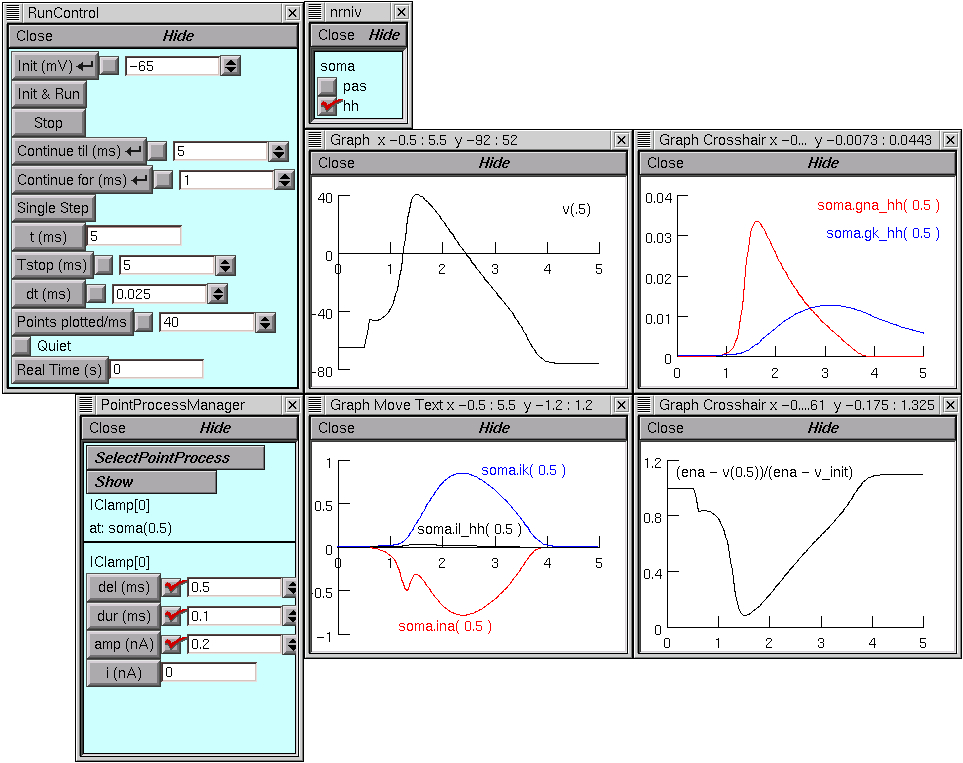
\includegraphics[height=\textheight,width=5in,keepaspectratio]{figures/neuron_gui.jpg}
\caption[The NEURON GUI \cite{brette2007simulation}]{The NEURON GUI showing the results of a simulation that has been run using the simulator\cite{brette2007simulation}.\label{fig:neuron_gui}}
\end{center}
\end{figure}

\begin{figure}
\begin{center}
\begin{lstlisting}
create soma, dend, dendx, axon
connect dend(0), soma(1)
connect dendx(0), soma(1)
connect axon(0), soma(0)

access soma
pt3dclear()
pt3dadd(0, 0, 0, 8)
pt3dadd(6, 0, 0, 18)
pt3dadd(10, 0, 0, 20)
pt3dadd(14, 0, 0, 18)
pt3dadd(20, 0, 0, 10)

insert hh
Ra = ra

dend {
  nseg = 21	// may need more
  diam = DEND_DIAM
  L = DEND_LENGTH

  insert hh
  gnabar_hh /= 5
  dend_gnabar_0 = gnabar_hh
  gkbar_hh /= 5
  Ra = ra
}
\end{lstlisting}
\caption[NEURON Hoc Example \cite{carenvale2006neuron}]{A code snippet from a Hoc script creating a neuron\cite{carenvale2006neuron}.\label{fig:hoc_example}}
\end{center}
\end{figure}

Another simulator, called GENESIS (GEneral NEural SImulation System)\cite{brette2007simulation}, is similar to NEURON in that it mostly models smaller neural networks including interactions within a single neuron\cite{bower1995book}. GENESIS uses a proprietary scripting language as well as formatted data files to create and run simulations. GENESIS can use MPI or PVM to parallelize its computations across multiple machines. Like NEURON, it can run simulations via a command-line interface known as G-Shell, a Python wrapper library, or a graphical user interface named XODUS\cite{brette2007simulation}. An example of the XODUS user interface can be found in Figure \ref{fig:genesis_gui} and a sample of the GENESIS scripting language can be found in Figure \ref{fig:gscript_example}\cite{bower1995book, brette2007simulation}.

\begin{figure}
\begin{center}
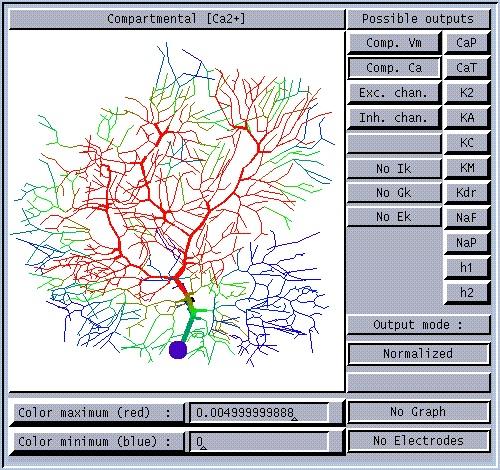
\includegraphics[height=\textheight,width=5in,keepaspectratio]{figures/genesis_gui.jpg}
\caption[The GENESIS GUI \cite{brette2007simulation}]{The GENESIS GUI (called XODUS) showing a visual representation of a Purkinje neuron model\cite{brette2007simulation}.\label{fig:genesis_gui}}
\end{center}
\end{figure}

\begin{figure}
\begin{center}
\begin{lstlisting}
create cell /n  
create segment /n/soma  
 
model_parameter_add /n/soma Vm_init -0.068  
model_parameter_add /n/soma CM 0.0164  
model_parameter_add /n/soma RM 1.500  
model_parameter_add /n/soma RA 2.500  
model_parameter_add /n/soma ELEAK -0.080  
 
model_parameter_add /n/soma LENGTH 4.47e-5  
model_parameter_add /n/soma DIA 2e-5  
 
runtime_parameter_add /n/soma INJECT 2e-9  
output_add /n/soma Vm  
 
run /n 0.05  
 
quit
\end{lstlisting}
\caption[GENESIS Script Example \cite{bower1995book}]{A code sample from a GENESIS script creating a neuron, injecting current into it, and outputting the voltage\cite{bower1995book}.\label{fig:gscript_example}}
\end{center}
\end{figure}

Unlike the NEURON and GENESIS simulators, the NEST (NEural Simulation Tool)\cite{brette2007simulation} simulator tends to focus on larger neural networks rather than smaller ones. NEST uses a command-line interface as well as a Python wrapper to create models and run simulations.  Unlike its counterparts, NEST lacks an out-of-the-box user interface component. Results of the simulation must be viewed using 3rd party Python libraries like matplotlib\cite{brette2007simulation}. An example of the NEST scripting language can be found in Figure \ref{fig:nest_script_example}\cite{gewaltig2007nest}.

The last simulator (and perhaps most-similar to NCS) that will be discussed is BRIAN. BRIAN is a neural simulator developed naively in Python and does not use a command-line intermediary: models are written exclusively in Python \cite{goodman2013brian}. BRIAN uses the scipy and numpy libraries to speed computations by taking advantage of native C code execution. It does not, however, provide the ability to parallelize the simulation across multiple machines. An example of a simple BRIAN simulation script can be found in Figure \ref{fig:brian_example}\cite{goodman2013brian}.

A comparison of these simulators and their features can be found in Table \ref{table:sim_comparison}\cite{hoang2013novel}.

\begin{figure}
\begin{center}
\begin{lstlisting}
/iaf_neuron Create /n1 Set
/iaf_neuron Create /n2 Set
/iaf_neuron Create /n3 Set
n1 n2 Connect
n1 n3 Connect
\end{lstlisting}
\caption[NEST Script Example \cite{gewaltig2007nest}]{A small code snippet of a NEST script creating three neurons and connecting them in a chain\cite{gewaltig2007nest}.\label{fig:nest_script_example}}
\end{center}
\end{figure}

\begin{figure}
\begin{center}
\begin{lstlisting}
from brian import *
eqs = '''
dv/dt = (ge+gi-(v+49*mV))/(20*ms) : volt
dge/dt = -ge/(5*ms) : volt
dgi/dt = -gi/(10*ms) : volt
'''
P = NeuronGroup(4000, eqs, threshold=-50*mV, reset=-60*mV)
P.v = -60*mV
Pe = P.subgroup(3200)
Pi = P.subgroup(800)
Ce = Connection(Pe, P, 'ge', weight=1.62*mV, sparseness=0.02)
Ci = Connection(Pi, P, 'gi', weight=-9*mV, sparseness=0.02)
M = SpikeMonitor(P)
run(1*second)
raster_plot(M)
show()
\end{lstlisting}
\caption[BRIAN Example \cite{goodman2013brian}]{An example of a BRIAN script creating a group of 4000 neurons and creating a raster plot from the result of the simulation\cite{goodman2013brian}.\label{fig:brian_example}}
\end{center}
\end{figure}

\begin{table}
\def\arraystretch{1.5}
{\tiny
\begin{tabular}{ l | p{0.5in} | p{0.5in} | p{0.60in} | l | p{0.70in} | p{0.5in} | p{0.50in} | p{0.4in} }
Simulator & Platform & Language & Coding Style & GUI & Realtime \newline Visualization & Neuron Models & Parallel Support & Python Interface \\
\hline
BRIAN & Linux Mac Windows & Python & Python & No & No & LIF HH IZH & None & Yes \\
\hline
GENESIS & Linux Mac Windows & C & C & Yes & No & HH & MPI PVM & No \\
\hline
NEURON & Linux Mac Windows & C C++ FORTRAN & HOC Python & Yes & No & HH LIF & MPI & Yes \\
\hline
NCS & Linux & C++ CUDA Python & Python & Yes & Under Development & HH LIF IZH & MPI GPU (ZeroMQ planned) & Yes \\
\hline
NEST & Linux Mac Windows & C++ Python & Python SLI & No & No & HH LIF IZH AdEx MAT2 & MPI & Yes \\
\hline

\end{tabular}
}
\caption[Simulator Comparison \cite{hoang2013novel}]{This table provides a comparison between the major neural simulators including NCS based on the features they provide users (modified from \cite{hoang2013novel}).\label{table:sim_comparison}\vspace{0.25in}}
\end{table}

\section{NCS}

NCS is a spiking neuron simulator that is written in C++ and CUDA. The simulator, similar to the BRIAN simulator discussed earlier, its currently focused on simulating large-scale neural networks, on the order of hundreds of thousands to millions of neurons and billions of synapses\cite{hoang2013novel, thibeault2011novel}. To handle these large-scale simulations, NCS is designed to scale to handle the sizable computational throughput needed. It is designed from the ground up to distribute the workload across multiple processors on multiple machines. In addition to using multiple CPU cores on each node, NCS also will detect and use NVIDIA GPUs if they are present on the machine to take advantage of the SIMD capabilities of these cards as well as their floating-point performance\cite{thibeault2011novel}.

Running on top of the C++ code is a thin Python layer that provides lower-level access to the simulator. This layer doesn't attempt to provide advanced capabilities in an effort to keep the C++ code as streamlined and as simple as possible without having to add additional overhead for higher-level functionality. For example, NCS doesn't explicitly provide any form of grouping or organization for the neurons it simulates. Rather, it keeps track of groups of neurons, individual neurons, and the connections between them. This may work for smaller simulations, but at the scale of millions of neurons and billions or trillions of synapses, this approach to organization would leave most users lost in their own design. Similarly, a thin python layer without programming conveniences like classes removes a level of abstraction that would be expected from a normal programmatic API. In addition, neuroscientists might like to avoid coding altogether and focus on the biology.

To provide an intuitive and modern way for neuroscientists to interact with the NCS simulator, a more capable and user-friendly interface needs to be created. Additionally, to make the simulator more extensible as a cluster-based neural simulator running large-scale models, a better method is needed to organize, create, run, manage, store, and report on simulations than running the simulation via a shell on the cluster and directly manipulating the filesystem. These characteristics of NCS and other neural simulators do not help them create collaborative environments where experiments can be shared, recreated, and verified. A better approach is needed to handling the many tasks that surround these simulators.

\section{Client-Server Model}

To solve these shortcomings, we have created a client-server based approach to the design of NCS. In this model of computing, a server running on a machine accepts requests from clients who wish to use the servers resources. A diagram of the client-server model can be found in Figure \ref{fig:client_server}\cite{wiki:clientserver}. In the context of NCS, the server will run on the master node of an NCS cluster and directly interface with the low-level Python interface. The server is responsible for multiple functions. Firstly, the server should be able to manage and keep track of the simulator. This includes calling NCS to run a simulation, ensuring that clients don't attempt to run a simulation while another is in progress, and managing the output of the simulator including resulting data, errors, warnings, and other messages as well as allowing clients to get access to this information. Using this computation model as opposed to the methods used by existing simulators provides a number of advantages. Firstly, the simulator can be used by multiple remote clients. This allows many different researchers to use the same cluster, and allows simulations to be run from non-console clients, such as a web browser. Secondly, it removes the need for direct shell access to the machine, which removes potential security risks associated with providing a remote shell. Lastly, it provides a centralized management system in which simulations can be logged, stored and shared in a consistent format, rather than the typical approach of allowing each user to create their own organizational methods. This makes it easier to share results, duplicate experiments, and incorporate models from other researchers into your own experiments.

\begin{figure}
\begin{center}
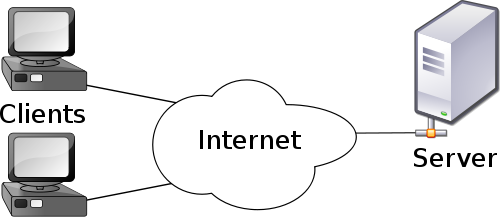
\includegraphics[height=\textheight,width=5in,keepaspectratio]{figures/client_server.png}
\caption[Client-Server Model \cite{wiki:clientserver}]{The client server model allows for multiple clients to request resources from the server\cite{wiki:clientserver}.\label{fig:client_server}}
\end{center}
\end{figure}

\section{HTTP \& REST}

\subsection{HTTP}

As a result of the client-server architecture chosen for NCS, a method is needed to transport information from the client to the server and vice versa. The HTTP protocol is a time-tested protocol used to transport textual and binary data over the Internet and various other computer networks. This makes HTTP an ideal candidate for handling the transfer of information between the client and server.

A HTTP transaction begins with a request from the client to the server. Each request can be one of four types: GET, POST, PUT, and DELETE. Each of these methods requests the server to perform a specific action on a target. The target of the action is specified as the \emph{path}. The path is specified like a UNIX filesystem path, in the form of a series of strings separated by forward slashes. The effect of actions GET, POST, PUT, and DELETE on a path are defined by the HTTP server itself, but generally follow a certain format\cite{fielding1999hypertext}. The GET method instructs the server that the client is requesting information about the path included in the request. For example, when visiting a website, a GET request to the path of / would ask the server to provide information pertaining to the index of the site, whereas a GET request to the path /blog would request information about the websites blog (provided such a path exists on the server). A POST request to /blog might instruct the server to create a new blog post with the data provided with the request (such as a title, author, and content).

Typically, when browsers interact with websites the data returned from the server is HTML, which the browser uses to render the page in the browser window. However, HTML is far from the only type of information that an HTTP response can contain. HTTP responses can contain plain text, binary data (including images), XML documents, JSON objects, or any other user-defined format. Following the standardization of HTTP/1.1 in 1999, which added the PUT and DELETE methods, HTTP became capable of performing all CRUD (Create, Read, Update, Delete) operations for persistent storage\cite{fielding1999hypertext}. The CRUD options of HTTP/1.1 form the basis of the REST architectural style\cite{fielding2000representational}.

\subsection{REST}

REST (REpresentational State Transfer) is an architectural pattern that defines a method of interaction between a client and server. The key component behind the REST architecture is the concept of a {\em{resource}}. A REST resource, in the context of HTTP, is a URI, or Uniform Resource Identifier. A URI for a web application is typically the location of the resource on the web server in the form of a URL or Uniform Resource Location\cite{fielding2000representational}. For example, the URI for the users resource might be http://example.com/users and a URI for a student who's student ID is 1033 might be http://example.com/student/1033. These URI's uniquely identify their respective resources on the servers they are hosted on as well as the Internet as a whole.

While the URI specifies a way to uniquely identify a resource, a method is needed to represent the resource\cite{fielding2000representational}. This is typically done using one of the formats mentioned in the previous section such as HTML, XML, or JSON. For example, a student resource might be represented in JSON format shown in Figure \ref{fig:json_example} or in an XML format such as in Figure \ref{fig:xml_example}. These formats provide a consistent method of interaction between client and server.

To interact with a RESTful interface in the context of HTTP, the client sends a request to a particular URI on the server with one of the HTTP methods mentioned previously. Sending a GET request tells the server that the client wishes to receive the representation of the resource it requested. If the client wished to receive the representation of the aforementioned student with ID 1033, it would send a GET request to the URI http://example.com/student/1033 and the server would respond with the information shown in Figure \ref{fig:json_example}. To add a student, the client would send a POST request to the server containing the representation of the student (in the same format as Figure \ref{fig:json_example}) directed at the URI corresponding to the new student's ID, say 1555, at http://example.com/student/1555. To update the student with ID 1555, the client would send a PUT request to the URI http://example.com/student/1555 with the updated user representation. Similarly, to remove the student, the client would send send a DELETE request to the URI http://example.com/student/1555. This architectural style makes a HTTP API standardized and predictable, making it easy for clients to interact with the server.

\section{The JSON Format}

There are several ways to transmit information over HTTP, some of which are discussed in the HTTP section of this chapter. The JSON (JavaScript Object Notation) format, as its name suggests, is derived from the Javascript syntax for an object. JSON, which was defined in 2001 by Douglas Crockford, is a textual format that takes a minimal approach to representing data\cite{bray2013json}. Unlike XML, JSON doesn't use opening and closing tags, but uses a list of properties instead, making the files smaller\cite{nurseitov2009comparison}. Additionally, JSON has several datatypes, which is a feature not present in XML, making it easily parsed into programming languages such as Python, Ruby, and Javascript, which usually require a single function call to turn a string of JSON into a language-native object. JSON also has a binary format called BSON that can be used to transfer and store information in a binary format that is more space conscious and holds a superset of the normal JSON data types\cite{chodorow2013mongodb}.

There are six data types available in the JSON format: number, string, boolean, array, object, and null\cite{bray2013json}. All strings in JSON are enclosed within double-quotes and are UTF-8 encoded. A JSON object is an associative array of name/value pairs, enclosed within curly braces. The names must be strings followed by a colon and then the value. The key/value pairs are delimited by commas. Numbers are decimal numbers that can be in E notation or fractional. Arrays are lists of values within square brackets delimited by commas. Boolean values are simply true and false, and null is represented as the text null. An example JSON document using all types is shown in Figure \ref{fig:json_all_types}.

\begin{figure}
\begin{center}
\begin{lstlisting}
{
    "name": "Bob",
    "grade": "sophomore",
    "age": 24,
    "phone": "1+(775)555-5555"
}
\end{lstlisting}
\caption[JSON User Example]{This figure shows how a user might be defined using the JSON format. The student contains four attributes. Name, grade, and phone are string attributes, whereas age is a numerical attribute.\label{fig:json_example}}
\end{center}
\end{figure}

\begin{figure}
\begin{center}
\begin{lstlisting}[language=XML]
<student>
    <name>Bob</name>
    <grade>sophomore</grade>
    <age>24</name>
    <phone>1+(775)555-5555</phone>
</student>
\end{lstlisting}
\caption[XML Example]{This figure shows how a user might be defined using the XML format. Like the JSON example in Figure \ref{fig:json_example}, this student object contains four elements. XML doesn't provide the ability to dictate the type of elements, so all elements contain strings.\label{fig:xml_example}}
\end{center}
\end{figure}

\begin{figure}
\begin{center}
\begin{lstlisting}
{
    "company_name": "Planetary Express",
    "phone": "1+(800)555-5555",
    "manager": "Hubert Farnsworth",
    "company_net_worth": 0.0,
    "personnel": [
        "Phillip J. Fry",
        "Turanga Leela",
        "Hermes Conrad",
        "Amy Wong",
        "John Zoidberg",
        "Scruffy",
        "Bender Rodriguez"
    ],
    "total_deliveries": 100,
    "website": null,
    "is_profitable": false
}
\end{lstlisting}
\caption[JSON All Types]{This figure shows all valid JSON types. company\_name is a string, personnel is an array, total\_deliveries is a numerical value, website is a null value, and is\_profitable is a boolean value.\label{fig:json_all_types}}
\end{center}
\end{figure}

\section{WebSockets}

HTTP is a request-response protocol. It does not provide a method of streaming data between the client and server in a full-duplex fashion like that of TCP. To solve this problem, a new protocol was created that allows full-duplex communication via HTTP called WebSockets. WebSockets allow Javascript running on the client's browser to initiate a connection with a server in which both the client and the server can send data to one another simultaneously\cite{fette2011websocket}. This is helpful in many different applications where it would not be desirable to continuously request data from the server (polling) when there may not be any data that the client needs. When using WebSockets, the client can simply wait until the server has data to send and receive it asynchronously without constantly polling the server for it. This greatly reduces the network footprint of real-time HTTP-based applications and provides a much more intuitive interface for the exchange of data between client and server when such situation arise. For example, a web-based instant messaging client could use WebSockets to wait for incoming messages from the server and receive them as soon as they are ready, as opposed to constantly polling the server many times per second to check for new messages.

\section{MongoDB}

In recent years, a number of new database systems have been developed that do not rely on the traditional relational-model, which often use SQL as their database language. These databases are colloquially known as NoSQL databases in reference to the fact that they do not use SQL as a data management language\cite{lith2010investigating}. MongoDB is one of these databases. Instead us using tables and columns like in a traditional database it uses collections and documents\cite{chodorow2013mongodb}. Documents are JSON objects that are stored in a BSON format on disk. A collection is a list of documents, usually with a similar format (but this is not required). This type of database is advantageous because it doesn't require a strict schema with each attribute in its own column like in a SQL database\cite{chodorow2013mongodb}. This allows more flexibility in the way you want to store and retrieve your data. For example, storing the data shown in Figure \ref{fig:json_all_types} would require a few different tables in a well-designed SQL database. MongoDB becomes even more advantageous when the data your application works with is already in a JSON format. MongoDB uses Javascript as the language to manage the database data, which provides methods for CRUD operations as well as a few aggregate functions such as summation and average. More complicated queries require the use of a MapReduce programming model\cite{chodorow2013mongodb}. Database ORMs exist in many languages for MongoDB, so often times the user will never need to use Javascript to interact with the database and can use the language of their choice. Python contains a a library called MongoKit that performs this task\cite{tsoukalos2014using}.

\section{Client-Side Web Development}

\subsection{Bootstrap}

Over the years, the Internet and the World Wide Web have seen a massive expansion in size, ubiquity and utility. As the World Wide Web evolves, the way websites are built and designed also continues to evolve. Originally, websites were designed by hand and often took an exorbitant amount of time to design and implement. Adding to the problem, different browsers render web pages differently; even when the code is exactly the same, the differences can often times be dramatic. To combat this, a number or tools and frameworks have come about that aim to be both easy to use and cross-browser compatible\cite{lerner2012forge}. One of these frameworks is Bootstrap. 

Originally developed by Twitter for creating a consistent UI for internal tools, Bootstrap is a front-end framework that provides design templates that work across browsers and for various screen sizes (including mobile) and aims to provide a clean and aesthetic user interface. Web page elements such as forms, buttons, headers, tables, navigation, alerts, panels and numerous others are included in the Bootstrap package so developers don't have to create and style them themselves. Bootstrap includes a number of Cascading Style Sheet (CSS) rules to create and style the widgets and elements on the page, as well as a small amount of Javascript to make some of the elements interactive, such as the accordion component that shows and hides different panels in an accordion-like fashion. An example of a web page created with Bootstrap is shown in Figure \ref{fig:bootstrap_web_page} and some of the components Bootstrap contains can be found in Figure \ref{fig:bootstrap_components}\cite{bootstrap2014}.

\begin{figure}
\begin{center}
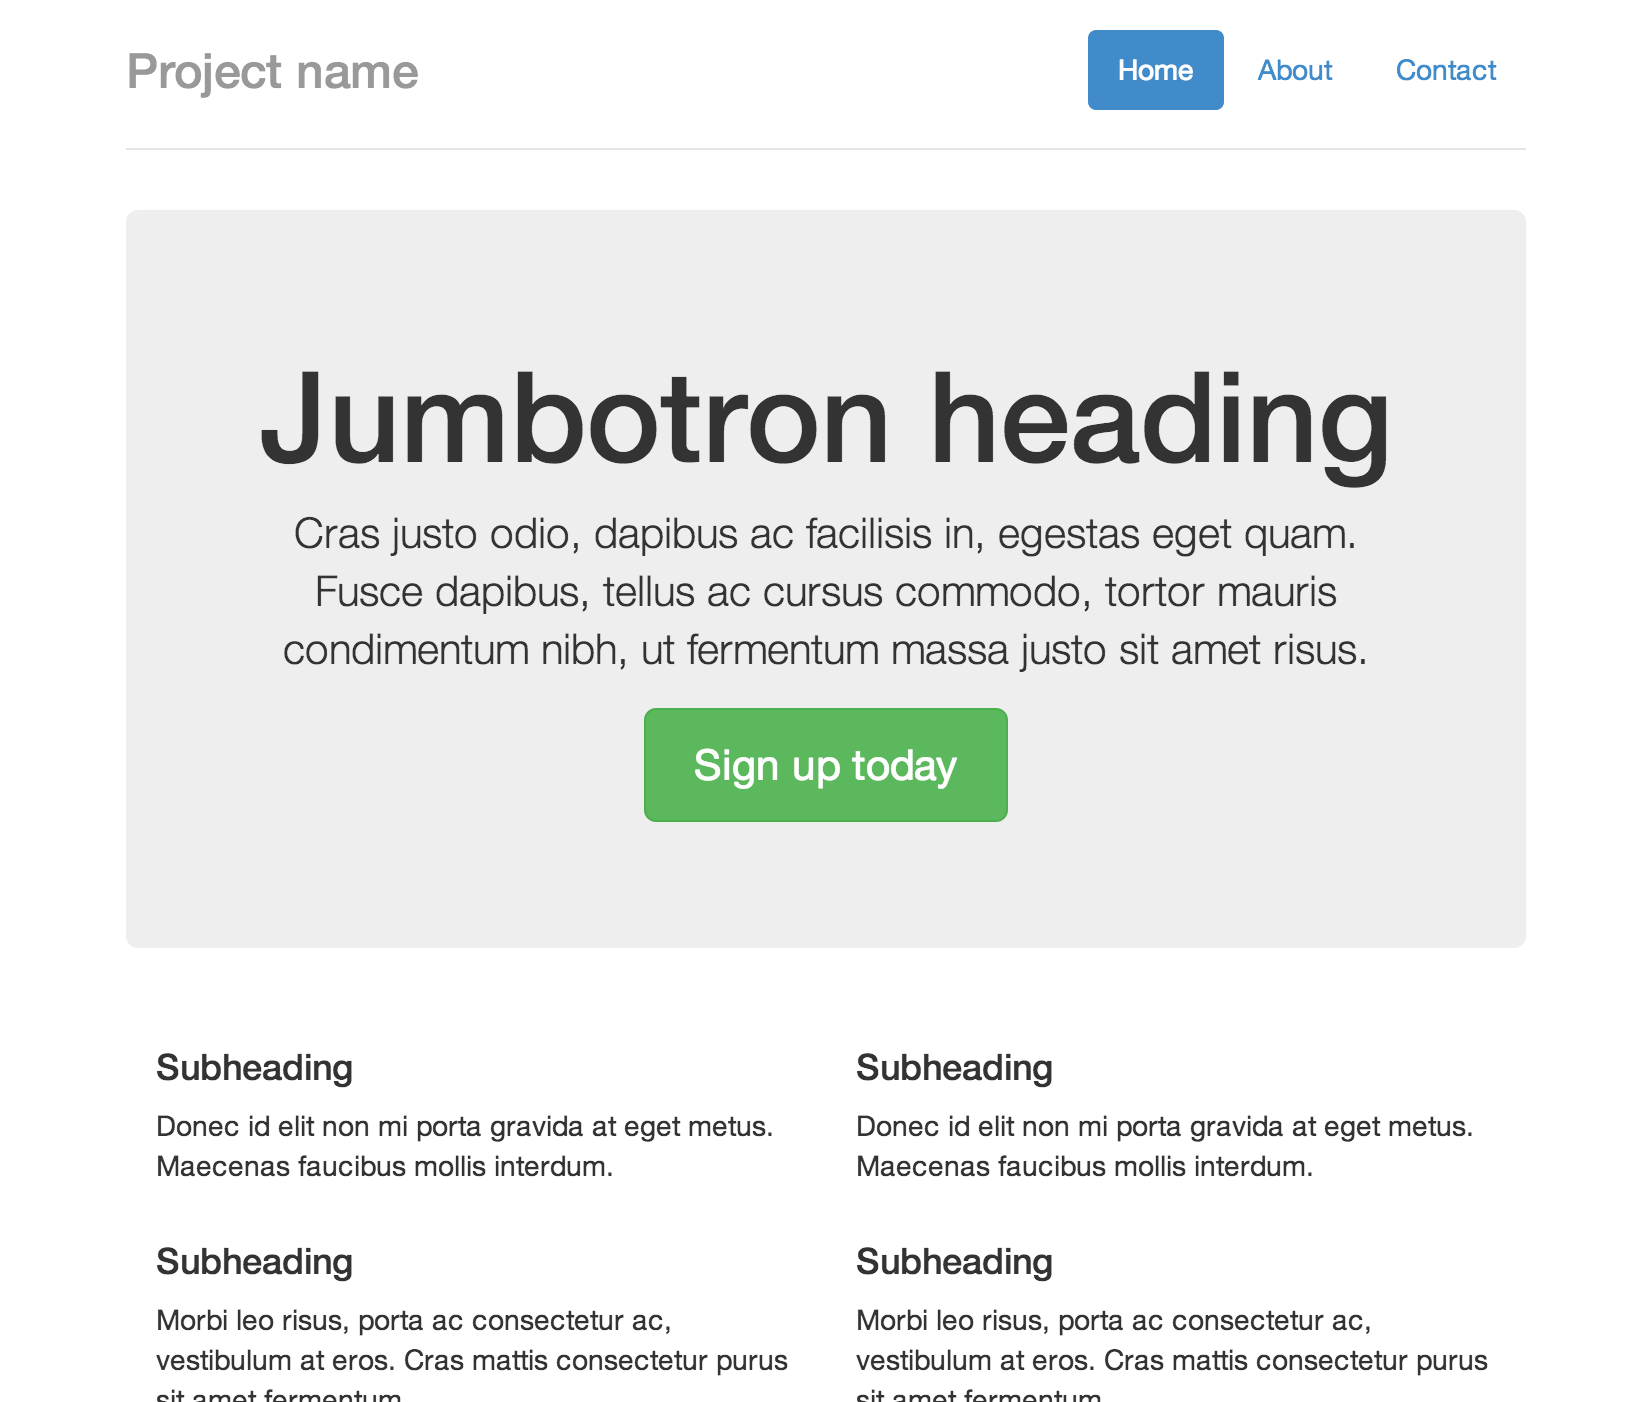
\includegraphics[height=\textheight,width=5in,keepaspectratio]{figures/bootstrap.png}
\caption[Bootstrap Web Page \cite{bootstrap2014}]{This is a simple example page that was created with the Bootstrap front-end framework. The page contains a navigation bar, page header, jumbotron component, and several paragraph elements that stack if the browser window becomes small enough\cite{bootstrap2014}.\label{fig:bootstrap_web_page}}
\end{center}
\end{figure}

\begin{figure}
\begin{center}
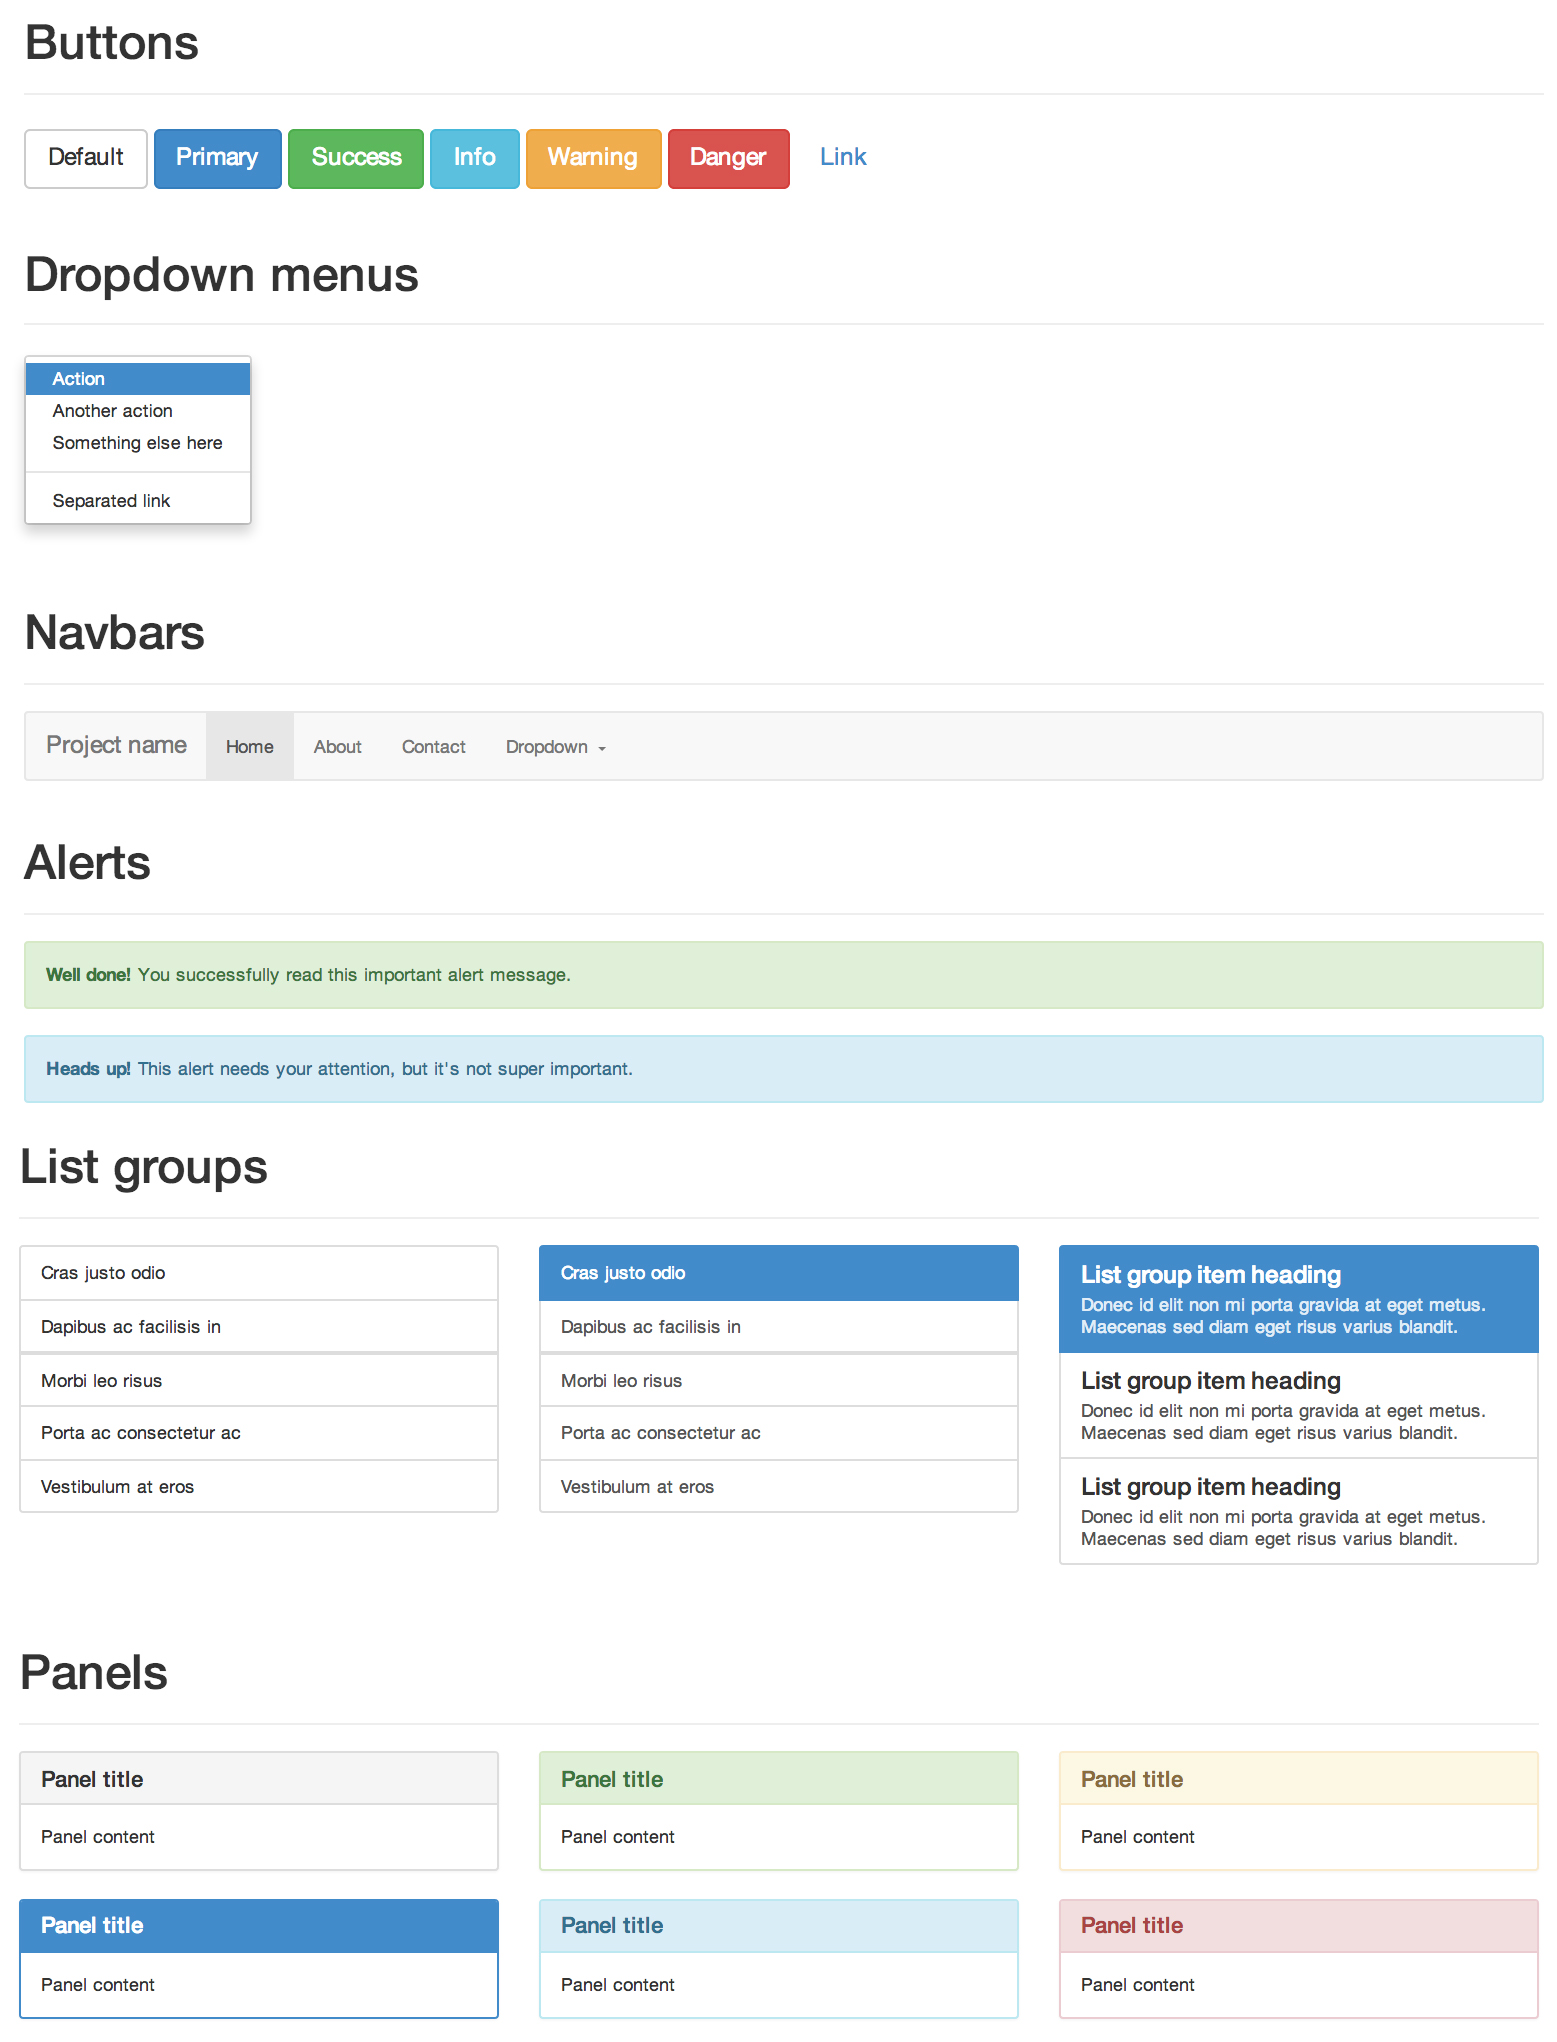
\includegraphics[height=\textheight,width=5in,keepaspectratio]{figures/bootstrap_components.jpg}
\caption[Bootstrap Components \cite{bootstrap2014}]{This figure shows several more Bootstrap components that are available for use in web applications\cite{bootstrap2014}.\label{fig:bootstrap_components}}
\end{center}
\end{figure}

\subsection{AngularJS}

While Bootstrap changes the way we create the look and feel of websites, AngularJS changes how we make web pages dynamic. Traditionally most of the code front-end developers would write involves directly manipulating the elements on the HTML page when data changes or the user interacts with the application. Most of this kind of development is tedious, and writing the code for it takes time away from other tasks that are central to the functionality of the application. Angular removes the need to write the code that manipulates the elements on the web page and allows developers to focus on the background tasks that need to be performed such as fetching data from a server\cite{darwin2013angularjs}. It does this by providing developers a way to create declarative-style directives in the HTML of the web page. An example of this would be rendering elements from a list on the page, such as a list of books. As books are added, deleted, and modified from a list in an Angular Javascript module, they are automatically updated on the web page instantly. This is a possible due to Angular's two-way data binding concept that is at the core of its functionality. As a result of the two-way data binding feature, any changes to the view are reflected in the model of the application, and any changes in the model are reflected in the view. A diagram illustrating this two-way data binding can be found in Figure \ref{fig:angular_data_binding}\cite{angularconcepts2014}. If you compare this with a traditional web application using jQuery to manipulate the DOM, you can see that the complexity of accomplishing a two-way data binding would greatly increase and would require you to write a lot more code. An example comparing the code required for each of these approaches can be found in Figure \ref{fig:jquery_example} and Figure \ref{fig:angular_example}.

Angular also provides a \emph{resource} module that allows developers to easily interact with RESTful interfaces. For each resource only requires a location be specified in the form of a URL where the resource can be found. Other options may be provided to enhance the behavior of the resource object in the event custom functionality may be needed, or in other cases when a list of objects might be returned instead of just a single object. This makes it trivial to create a Javascript application that interacts with a RESTful web application. An example of creating and using an Angular resource can be found in Figure \ref{fig:angular_resource}.

\begin{figure}
\begin{center}
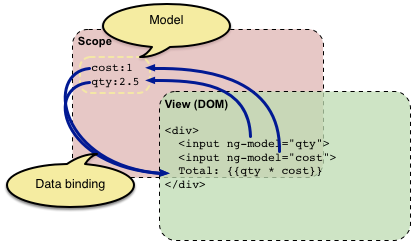
\includegraphics[height=\textheight,width=5in,keepaspectratio]{figures/angular_data_binding.png}
\caption[Angular data binding \cite{angularconcepts2014}]{This figure illustrates the concept of Angular's data-binding feature. Changes to the scope's cost and qty variables are automatically propagated to the view without any further action required by the developer. If the user changes the values in the input areas on the web page, those changes are automatically reflected in the scope variables as well\cite{angularconcepts2014}.\label{fig:angular_data_binding}}
\end{center}
\end{figure}

\begin{figure}
\begin{center}
\begin{lstlisting}
$.ajax({
  url: '/message_list',
  success: function (data, status) {
    var result = JSON.parse(data);
    for (var i = 0; i < result.length; i++) {
      $('ul#log').append('<li>' + result[i].msg + '</li>');
    }
  }
});
\end{lstlisting}
\begin{lstlisting}[language=HTML]
<ul class="messages" id="log">
</ul>
\end{lstlisting}
\caption[JQuery DOM Manipulation]{This Javascript snippet uses JQuery to perform an HTTP request to get some data from the server and add it to an HTML list. The Javascript code is highly dependent on the HTML code. The {\em{}`ul\#log'} provides a specific HTML element to add the element to. What if the data needed to be used in another HTML element? We would need to modify the request function.\label{fig:jquery_example}}
\end{center}
\end{figure}

%%%%%%%%%%%%%%%%%%%%%%%%%%%%%%%%%%%%%%%%%%%%%%%

\begin{figure}
\begin{center}
\begin{lstlisting}
$http( '/message_list' ).then( function ( response ) {
  for (var i = 0; i < response.length; i++) {
    $scope.log.push( response[i] );
  }
});
\end{lstlisting}
\begin{lstlisting}[language=HTML]
<ul class="messages">
    <li ng-repeat="entry in log">{{ entry.msg }}</li>
</ul>
\end{lstlisting}
\caption[Angular DOM Manipulation]{This Javascript snippet uses Angular to perform an HTTP request to get some data from the server and add it to an HTML list. The data being retrieved has no ties to the HTML code at all. In the HTML, we add an angular directive (ng-repeat) to loop over the list of messages and add the elements dynamically.\label{fig:angular_example}}
\end{center}
\end{figure}

\begin{figure}
\begin{center}
\begin{lstlisting}
var User = $resource('/user/:userId', {userId:'@id'});
User.get({userId: 1155}, function(user) {
  $scope.users.push(user);
});
\end{lstlisting}
\begin{lstlisting}

\end{lstlisting}
\caption[Angular Resource Module]{This figure demonstrates Angular's resource module. This module allows Angular to easily interact with RESTful web servers. The developer defines the Angular resource using the URL of the resource on the server. Once the resource has been defined, the developer can query the RESTful interface using the resource object.\label{fig:angular_resource}}
\end{center}
\end{figure}

